% !TEX TS-program = pdflatex
% !TEX encoding = UTF-8 Unicode

\documentclass[10pt,twocolumn]{article}

\usepackage{graphicx,listings,fixltx2e,lambda,array,times,fullpage}

\begin{document}

\title{Parakeet: A Just-In-Time Parallel Accelerator for Python}
\author{
Alex Rubinsteyn \ \ \ \ Eric Hielscher \ \ \ \ Nathaniel Weinman \ \ \ \
Dennis Shasha \\
{\it Computer Science Department, New York University, New York, NY, 10003} \\
\small{\tt \{alexr,hielscher,nsw233,shasha\} @ cs.nyu.edu}
}
\date{}

% define some useful commands to use in language specification 
\newcommand{\WITH}{\impfnt{with}}
\newcommand{\VALUES}{\impfnt{values}}
\newcommand{\MAP}{\impfnt{map}}
\newcommand{\REDUCE}{\impfnt{reduce}}
\newcommand{\ALLPAIRS}{\impfnt{allpairs}}
\newcommand{\CAST}{\impfnt{cast}}
\newcommand{\APPLY}{\impfnt{apply}}
\newcommand{\INDEX}{\impfnt{index}}
\newcommand{\SCAN}{\impfnt{scan}}
\newcommand{\THREADIDX}{\impfnt{threadIdx}}
\newcommand{\BLOCKIDX}{\impfnt{blockIdx}}
\newcommand{\BLOCKDIM}{\impfnt{blockDim}}
\newcommand{\GRIDDIM}{\impfnt{gridDim}}
\newcommand{\VEC}{\impfnt{vec}}
\newcommand{\concat}{\ensuremath{+\!\!\!\!+\,}}

\setlength\fboxsep{8pt}
\setlength\fboxrule{0.5pt}

\maketitle

\begin{abstract}
% Dennis's outline:
% 1. python as written
% 2. speedups for llvm
% 3. extensibility
% 4. speedups for gpus
% 5. vapor about how to unify

High level productivity languages such as Python or Matlab enable the use of computational resources by non-expert programmers.  However, these languages sacrifice program speed for ease of use, with this trade-off especially stark for modern parallel processors such as multicore CPUs and manycore GPUs.

In this paper, we discuss Parakeet, a library which provides a just-in-time (JIT) parallel accelerator for Python.  Parakeet bridges the gap between the usability of Python and the speed of code written in efficiency languages such as C++ or CUDA.  Parakeet accelerates data-parallel sections of Python that use the standard NumPy scientific computing library.  Parakeet automatically JIT compiles efficient versions of Python functions and manages their execution on both GPUs and multicore CPUs.  We assess Parakeet on a pair of benchmark programs and exhibit significant speedups.  We use these current results as a basis for discussing our plans to augment the Parakeet feature set.
\end{abstract}

\section{Introduction}
\label{Intro}

% What is the problem we're trying to solve?  Who should care about this paper?
Computational resources are indispensable tools to professionals in a wide range of fields, from the natural sciences to the financial industry.  Often, users in these fields either (1) aren't expert programmers; or (2) don't have time to spend on writing and tuning their software for performance.  Thus, these users typically prefer to use productivity languages such as Python or Matlab as opposed to efficiency languages such as C++.  Productivity languages facilitate non-expert programmers by trading off program speed for ease of use \cite{Pre03}.

A common problem, however, is that this tradeoff is often very stark -- code written in Python or Matlab~\cite{Moler80} often has much worse performance than code written in C++.  In addition, this problem is getting worse, as modern processors (both multicore CPUs as well as manycore GPUs) are all parallel, and current implementations of productivity languages are poorly suited for parallelism.  Thus a common workflow involves rapid prototyping of algorithms in a productivity language, followed by porting the performance-critical sections to an efficiency language so as to achieve tolerable performance.  This second step can be time-consuming, error-prone, and diverts energy from the real focus of these users' work.

% Heart of Parakeet - an interpreter for our high level IL w/ array ops
In this paper, we present Parakeet, a library that provides a JIT parallel accelerator for the commonly-used NumPy extensions for scientific computing~\cite{Oliphant07}. Parakeet accelerates performance-critical sections of numerical Python programs to be competitive with efficiency language code, obviating the need for the above-mentioned ``prototype, port'' cycle.

The Parakeet library intercepts functions that have been marked with a decorator, and uses the data-parallel array operations over NumPy arrays as sources of parallelism. These functions are just-in-time compiled to either x86 machine code using LLVM~\cite{Latt02}, or GPU programs that can be executed on NVIDIA GPUs via the CUDA framework~\cite{NvidCU}. These native versions of the functions are then automatically executed on the appropriate hardware. Parakeet allows complete interoperability with all of the standard Python tools and libraries.

While Parakeet is a work in progress, our current results clearly demonstrate its promise.  In the near future, Parakeet's CPU support will be extended to make better use of modern multicore processors.  Our vision for Parakeet includes eventual support for splitting computations across CPUs and GPUs simultaneously -- keeping all processors in a system busy at once -- and on-the-fly tuning of resource usage.

\begin{figure*}[t!bh]
\begin{center}
\leavevmode
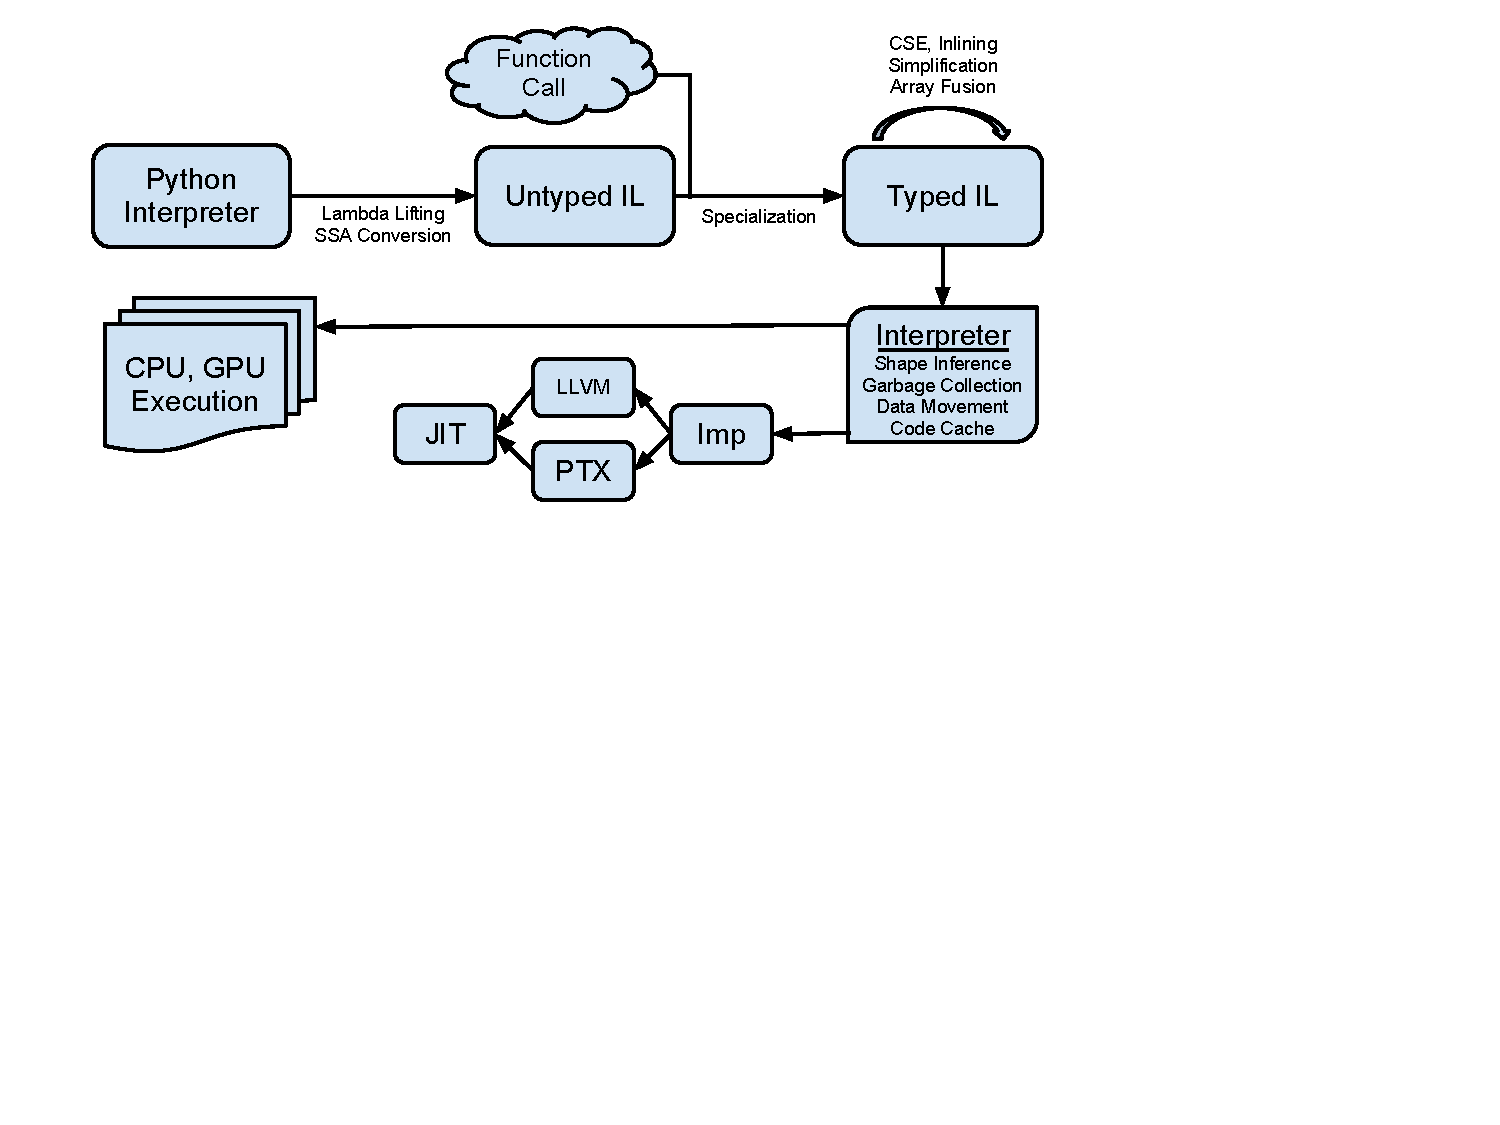
\includegraphics[scale=0.6, trim=0pt 310pt 140pt 80pt]{ParakeetNumPyOverview.pdf}
\end{center}
\caption{Parakeet Pipeline}
\label{fig:overview}
\end{figure*}

\section{Overview}
\label{overview}
%Might be useful: 
% array operations encode rich information about their access patterns that we can exploit to translate them into efficient parallel programs \cite{Ju94}.
Parakeet is an accelerator library for numerical Python programs written using the NumPy numerical computing library~\cite{Oliphant07}.  Parakeet accelerates entire functions at a time by just-in-time compiling native versions of the functions for execution on both GPUs and multicore CPUs.

Parakeet is not meant as a general-purpose accelerator for all Python programs.  Rather, it is designed to benefit numerically intensive algorithms (such as those used in machine learning, financial computing, scientific simulation, etc.).  In particular, the sections of code that Parakeet accelerates must obey the following constraints:

\begin{itemize}
 \item Only use scalar values or NumPy arrays.  No dictionaries, sets, or user-defined objects are allowed.
 \item Can't reassign any global variables (though other accesses are allowed).
%\item No I/O is allowed.
 \item For a given set of inputs to the function, Parkaeet must be able to infer a unique type for every variable in the function's body (i.e.~code such as that in Listing \ref{unique-types} is not allowed):
\end{itemize}
\begin{lstlisting}[numbers=none,label=unique-types,caption=Unique Types Example,language=Python,frame=single]
  def fun(x):
    if x:
      return 42
    else:
      return "sausage"
\end{lstlisting}

While these constraints may at first seem highly restrictive, it is important to keep two things in mind.  First, they are only constraints on the functions that he or she explicitly marks for Parakeet acceleration.  Such functions can coexist in a module with code that doesn't satisfy these constraints, and that code will be executed as normal by the Python interpreter.  Second, these constraints still allow for idiomatic data-parallel programming using NumPy.  In practice, most code requires little or no modifications.

\subsection{Code Example}
Let's make things more concrete with a code example.  Figure \ref{MinIdx} shows two functions that form part of the K-Means clustering benchmark we use to evaluate Parakeet in Section \ref{Evaluation}.  The \texttt{minidx} function takes two inputs: a matrix \texttt{C} of vectors, and another vector \texttt{x}.  It computes the index of the vector in \texttt{C} whose distance from \texttt{x} is the smallest.

The program execution pipeline for NumPy code by Parakeet (shown in Figure \ref{fig:overview}) begins in the standard Python interpreter. At program start time, a subset of the program's functions (annotated manually by the programmer with a function decorator) are registered with Parakeet as potentially accelerable. The body of a registered function is then translated into an untyped intermediate representation using the Parakeet front end interface and the Python's introspection facilities.

\begin{figure}[h!]
\begin{lstlisting}[numbers=none,language=Python,frame=single]
def sqr_dist(x,y):
  return sum((x-y) * (x-y))

@PAR
def minidx(C,x):
  sqr_dists = map(sqr_dist,C,fixed=[x])
  return argmin(sqr_dists)
\end{lstlisting}
\caption{Minimum Distance Example}
\label{MinIdx}
\end{figure}

When a call is made to a function which has been registered with Parakeet, the untyped function is specialized by propagating type information from the arguments to all values in the body.  Type specialization translates the function into a typed intermediate language. Further standard optimizations are performed at this stage, the most impactful of which is \emph{array operator fusion}, wherein array operations are combined according to rewriting rules. This fusion step can be extremely beneficial to the final program's performance, especially when executed on the GPU, as it can drastically increase computational density and eliminate many wasteful array temporaries.

Execution of the optimized typed IL is initiated by Parakeet's interpreter, which is then responsible for deciding which operations to JIT compile to native code for the CPU or GPU. When the interpreter encounters an array operator it employs a simple cost-based heuristic (which considers nested array operators, data sizes, and memory transfer costs) to decide where to execute it (for more details see Section \ref{costmodel}). Parakeet's interpreter invests great effort into analyzing both the program and information about the data to make dynamic execution decisions. The cost of these analyses are mitigated by the tremendous computational density of the intermediate language's array operators.

If an array operator's computation is deemed a good candidate for native hardware execution, Parakeet flattens all nested array computations within that operator into sequential loops.  This payload is then inlined into a program skeleton that implements that operator.  For example, in the case of a \textbf{map} operation, Parakeet provides skeletal algorithms that implement the pattern of applying the same function to each element of an array on the CPU as well as on the GPU.  The flattened payload function argument is inlined into this skeleton, and a complete program is synthesized and JIT compiled.

To execute the native code, Parakeet first copies any of its inputs that aren't already present in the memory of the target hardware to their necessary place.  Parakeet manually manages the memory of the system, for example treating the GPU's memory as a cache of data whose canonical values are the CPU's RAM. The program is then executed, with memory reclaimed via garbage collection.

\section{Translation, Specialization, and Optimization}
\label{Compilation}
Now we turn to the problem of compiling an array language program into an efficient GPU program. At first glance, there seems to be a significant mismatch between the highly dynamic expressiveness of an array language like Q and the limitations imposed by GPU hardware discussed in Section \ref{GPULimitations}. Indeed, the Parakeet intermediate language must serve as a compromise between two competing tensions. In order to translate array programs into efficient GPU code it is necessary for the compiler to eliminate as much abstraction as possible. On the other hand, we must be careful not to make our program representation overly concrete with regard to evaluation order (which would eliminate opportunities for parallelism provided by the array operators). 

In deference to the above-mentioned GPU hardware restrictions, any program which is compiled to run on the GPU cannot have any of the following:

\begin{itemize}
\item Polymorphism (over types, array ranks, etc..) 
\item Recursion
\item User-specified higher-order functions
\item Compound data types other than arrays
\end{itemize}

Some of these restrictions (such as recursion, use of compound data types) limit the set of programs which can be executed by Parakeets. Certain types of polymorphism and some uses of higher order functions, however, can be effectively eliminated by program transformations. We enumerate some of these transformations (such as lambda lifting and specialization) which help bridge the abstraction gap between an expressive dynamically typed language and the GPU hardware. We also demonstrate several optimizations which, while beneficial in any compiler, are particularly important when targeting a graphics processor. Seemingly small residual inefficiencies in our intermediate form can later manifest themselves as the creation of large arrays, needless memory transfers, or wasteful GPU computations.

\subsection{Lambda Lifting and SSA Conversion}
After a function call has been intercepted by the Parakeet runtime, Parakeet performs a syntax-directed translation from a language-specific abstract syntax tree (AST) into Parakeet's IL. Since type information is not yet available to specialize user functions, the functions must be translated into an untyped
form (by setting all type assignments to $\bot$). The translation into Parakeet's IL maintains a closure environment and a name environment so that simultaneous lambda lifting and SSA conversion can be performed.

Since we would like to interpret our intermediate language we use a gated SSA form based on the GSA sub-language of the Program Dependence Web \cite{Ott90}. Classical SSA cannot be directly executed since the $\phi$-nodes lack deterministic semantics. Gated SSA overcomes this limitation by using "gates" which not only merge data flow but also associate predicates with each data flow branch. Aside from simplifying certain optimizations, these gates also enable us to execute our code without converting out of SSA.  For the sake of clarity, we elide SSA gates from the specifications of our untyped and typed intermediate languages. 

Figure \ref{UntypedSSADist} shows the \texttt{dist} function after it has been translated to Untyped SSA.

\begin{figure}[h!]
\fbox{
\begin{tabular}{ m{0.1cm} m{6.7cm} }
  \multicolumn{2}{l}{dist $($ x, y $) \rightarrow  ($ z $) =$} \\
  & t$_1 = \mathrm{x} - \mathrm{y} $        \\
  & t$_2 = \mathrm{x} - \mathrm{y} $        \\
  & t$_3  = \mathrm{t}_1 * \mathrm{t}_2 $   \\
  & t$_4  = $sum$(\mathrm{t}_2) $           \\
  & z $  = \; \mathrm{sqrt}(\mathrm{t}_4)$   \\
\end{tabular}
}
\caption{Untyped Distance Function in SSA form}
\label{UntypedSSADist}
\end{figure}

\subsection{Untyped Optimizations}
Parakeet performs optimizations both before and after type specialization. We subject the untyped representation to inlining, common subexpression elimination and simplification (which consists of simultaneous constant propagation and dead code elimination). This step occurs once for each function, upon its first interception by Parakeet. It is preferable to eliminate as much code as possible at this early stage since an untyped function body serves as a template for a potentially large number of future specializations. The only optimizations we do not perform on the untyped representation are array fusion rewrites, since these rely on type annotations to ensure correctness.

In our distance example, untyped optimizations will both remove a redundant subtraction and inline the definition of the $sum$ function, which expands to a $\REDUCE$ of addition.
\begin{figure}[h!]
\fbox{
\begin{tabular}{ m{0.1cm} m{6.7cm} }
  \multicolumn{2}{l}{dist $($ x, y $) \rightarrow  ($ z $) =$} \\
  & t$_1 = \mathrm{x} - \mathrm{y} $        \\
  & t$_2  = \mathrm{t}_1 * \mathrm{t}_1 $   \\
  & t$_3  = \REDUCE(+, 0, \mathrm{t}_2) $    \\
  & z $  = \; \mathrm{sqrt}(\mathrm{t}_3)$   \\
\end{tabular}
}
\caption{Distance Function after untyped optimizations}
\end{figure}

\subsection{Specialization}
Specialization transform user programs from the untyped intermediate language into its typed variety. The purpose of this transformation is to eliminate polymorphism, to make manifest all implicit behavior (such as coercion and scalar promotion), and to assign simple unboxed types to all data used within a function body. Beyond the fact that the GPU requires its programs to be statically typed, these goals are also essential for the efficient execution of user code on the GPU. Thus, the specializer generates a different specialized version of a function for each distinct call string, with all of the function's variables receiving the appropriate types.

\begin{figure}[h!]
  \begin{tabular}{| m{0.01cm}m{1.3cm}m{0.1cm}m{0.2cm}p{5.0cm} |}
  \hline
    & & & &\\
   \multicolumn{5}{|l|}{\textbf{Typed First-Order IL}}  \\[4pt]
  & program & $p$ &  $\bnfdef$   &  $d_1 \cdots d_n $ \\[4pt]
  & definition & $d$ & $\bnfdef$ & $f_i(x^m : \tau^m) \rightarrow (y^n : \tau^n) = \overline{s} $ \\[4pt]
  & statement  & $s$ & $\bnfdef$ & $x^m : \tau^m = e $\\[2pt]
  &            &     & $\sep$    & $\mathrm{if} ~v~ \mathrm{then} ~\overline{s}~ \mathrm{else} ~ \overline{s}$ \\[2pt]
  &            &     & $\sep$    & $\mathrm{while} ~ \overline{s}, x_{cond} ~ \mathrm{do} ~ \overline{s} ~  $ \\[4pt]
  & expression & $e$ & $\bnfdef$ & $\mathrm{values}(\overline{v})$ \\[2pt]
  &            &     & $\sep$    & $\mathrm{cast} (v, \tau_{src}, \tau_{dest})$ \\[2pt]
  &            &     & $\sep$    & $\mathrm{prim}_{\left\langle \oplus \right\rangle }(\overline{v})$ \\[2pt]
  &            &     & $\sep$    & $\mathrm{call}_{\left\langle f  \right\rangle } (\overline{v})$ \\[2pt] 
  
  &            &     & $\sep$    & $\MAP _{\left\langle c \right\rangle}(\overline{v})$ \\[2pt]
  &            &     & $\sep$    & $\REDUCE _{ \left\langle c_i, c_r \right\rangle } (\overline{v_i}, \overline{v})$ \\[2pt]
  &            &     & $\sep$    & $\SCAN _{ \left\langle c_i, c_r, \right\rangle} (\overline{v_i}, \overline{v})$ \\[5pt]
  & value      & $v$ & $\bnfdef$ & numeric constant \\[2pt]
  &            &     & $\sep$    &  $x$  \quad \small{(data variable)} \\[2pt]
  & closure    & $c$ & $\bnfdef$ & $f \times \overline{v}$ \\[4pt]
  & type & $\tau$    & $\bnfdef$ & $bool \sep int \sep float \sep \mathbf{vec} \; \tau   $\\[5pt]
  \hline
  \end{tabular}\\[4pt]
  \caption{Typed First-Order Language}
  \label{TIL}
\end{figure} 

A specification of our intermediate language is shown in Figure \ref{TIL}. We take inspiration from \cite{Bol09} and allow functions to both accept and return multiple values. This feature simplifies the specification of certain optimizations and naturally models the simultaneous creation of multiple values on the GPU. By convention we will write $\overline{\tau_m}$ to denote a sequence of $m$ simple types, $\overline{v_n}$ for a sequence  of $n$ values, etc. A single element is equivalent to a sequence of length 1 and sequences may be concatenated via juxtaposition, such that $\tau, \overline{\tau_n} = \overline{\tau_{m+1}}$.

The array operators $\MAP$, $\REDUCE$, and $\SCAN$ form a carefully confined higher-order subset of our otherwise first-order language and thus we elevate them to primitive syntax. These operators are important since they are the only constructs in our language that we attempt to parallelize automatically through GPU code synthesis. This isn't to say these are the only constructs executed in parallel on the GPU. The simple (first-order) array operators such as \textbf{sort} can be executed in parallel on the GPU as well via a fixed parallel standard library. 


It is important to note that uncertainty with regard to function values has been made completely explicit in this intermediate language. Every higher-order operator carries known labels for its function arguments. Any uncertainty in the original source must be directly encoded as an enumeration over a finite set of possible function calls. Function labels are associated with a set of closure argument values, which are necessary in order to support partial function application. This representation of function values resembles defunctionalization combined with specialization of \textit{apply} functions \cite{Tolmach98}. 

In order for higher-order functions to be translated into the Parakeet IL, it must be possible to specialize away all higher-order arguments. There are situations where exhaustive specialization is not possible (e.g. combinator libraries); in these cases, we revert to the source language's interpreter for
execution. This highlights an important point: since Parakeet augments (but does not replace) the interpreter of the source language, we are free to disallow problematic language constructs.



To continue the example, if the \textit{dist} function is called with arguments of type $vec~ float$ the specializer will then generate the code shown in Figure \ref{SpecDist}.
\begin{figure}[h!]
\fbox{
  \begin{tabular}{m{0.1cm} m{6.7cm}}
    \multicolumn{2}{l}{dist $($ x $ : vec \; float $, y : $ vec \; float $) $
\rightarrow  ($ z $ : float ) =$}  \\
    & t$_1   = \MAP ( -_{\mathrm{float}}, \mathrm{x}, \mathrm{y})$   \\
    & t$_2   = \MAP (*_{\mathrm{float}}, \mathrm{x}, \mathrm{y})$    \\
    & t$_3 = \REDUCE (+_{\mathrm{float}}, 0, \mathrm{t}_2)$          \\
    & z $  = \; \mathrm{sqrt}(\mathrm{t}_3)$                         \\
  \end{tabular}
}
\caption{Distance Function After Specialization}
\label{SpecDist}
\end{figure}

The actual intermediate language associates type annotations with every binding, which we elide here for clarity. Note that the polymorphism inherent in math operations between dynamically typed values has been removed through the use of statically typed math operators, and implicit \textbf{map}s on vectors (such as the subtraction between $x$ and $y$) have been expanded and made explicit.

\subsection{Array Operator Fusion}
In addition to standard compiler optimizations (such as constant folding, function inlining, and common sub-expression elimination), we employ fusion rules~\cite{Jones01} to combine array operators. Fusion enables us to minimize kernel launches, boost the computational density of generated kernels, and avoid the generation of unnecessary array temporaries.

We present the fusion rules used by Parakeet in simplified form, such that array operators only consume and produce a single value. Our rewrite engine actually generalizes these rules to accept functions of arbitrary input and output arities.
\\[5pt]
\begin{tabular}{|m{0.001cm} m{0.05cm} p{6.75cm} p{0.05cm} |}
  \hline 
  & &  & \\
  & \multicolumn{2}{l}{\large{Map Fusion} }  &  \\[2.5pt]
  & & $\MAP(g, \MAP(f, x)) \leadsto \MAP(g \circ f, x)$ & \\
  & & & \\
  & \multicolumn{2}{l}{\large{Reduce-Map Fusion} }  & \\[2.5pt]
  & & $\REDUCE(g_r, g_{i}, \MAP(f, x)) \leadsto \REDUCE(g_r \circ f, g_{i} \circ f, x)$ & \\
  & & & \\
  \hline
\end{tabular}\\[4pt]
These transformations are safe if the following conditions hold:
\begin{enumerate}
\item All the functions involved are referentially transparent.

\item Every output of the predecessor function ($f$) is used by the successor
($g$).

\item The outputs of the predecessor are used \textit{only} by the successor.
\end{enumerate}
The last two conditions restrict our optimizer from rewriting anything but linear chains of produced/consumed temporaries. A large body of previous work~\cite{Ald01} has demonstrated both the existence of richer fusion rules and cost-directed strategies for applying those rules in more general scenarios. Still, despite the simplicity of our approach, we have observed that many wasteful temporaries in idiomatic array code are removed by using only the above rules.

In Figure \ref{DistFuse}, we see the resulting optimized and specialized \texttt{dist} function. The two \textbf{map}s have been fused into the \textbf{reduce} operator, with a new function $f_1$ generated to perform the computation of all three original higher-order operators.

\begin{figure}[h!]

\fbox{
  \begin{tabular}{m{0.1cm} m{6.7cm} }
    \multicolumn{2}{l}{$\mathrm{f}_1 ($ acc : $ float $,  x $ : float $, y : $ float $) $ \rightarrow  ($ z $ :  float ) =$} \\
    & t$_1 = x - y $            \\
    & t$_2  = t_1 * t_1 $       \\
    & z $ = $ acc $+$ t$_2$     \\
    &  \\ 
  \multicolumn{2}{l}{$\mathrm{dist} ($~x $ : vec \; float $, y : $ vec \; float
$) $ \rightarrow  ($ z $ : float ) =$} \\
  & t$_3 = \REDUCE (\mathrm{f}_1, 0.0, \mathrm{x}, \mathrm{y})$   \\
  & z $ = \mathrm{sqrt}(\mathrm{t}_3)$  \\
  \end{tabular}
}
\caption{Distance Function After Fusion Optimization}
\label{DistFuse}
\end{figure}

\section{The Parakeet Runtime}
\label{runtime}

Once a function has been type specialized and fully optimized, it is handed off to the Parakeet runtime for intelligent execution. The heart of the runtime is a heavy-weight interpreter whose primary responsibility is to initiate GPU kernel synthesis and execution. The interpreter uses program analyses and performance heuristics in order to dynamically make decisions such as: 
\begin{enumerate}
\item what portion of a user's program ought to run on the GPU 
\item which level of nested parallelism ought to expressed as a GPU kernel
\item in which GPU memory space should a particular array reside 
\item when should data be moved onto or off the GPU
\end{enumerate} 

\subsection{Cost Model}
\label{costmodel}

When the Parakeet interpreter encounters an array operator, it uses a simple cost model to decide what is the best place to execute the operator.  The cost model employs a recursive function that estimates the relative cost of executing that operator on the CPU versus the GPU.  This function is not meant to measure the precise expected run time of the operator; rather, the goal is to make the correct decision when the use of one or the other processor should result in much higher performance.  We use the clock frequency of each processor to roughly estimate the cost of a single operation.  For each array operator, we multiply the estimated cost of a single execution of the operator's function argument by some fixed function of the input size.  For a \textbf{map} operation, for example, we multiply the estimated cost of performing the sequentialized version of the mapped function by the number of input elements. In addition, we estimated the time needed to transfer data to and from the GPU as a function of data size and add this cost to the total if the data is not already present in the respective processor's memory.

In the case of nested array operators -- e.g.~a \textbf{map} whose payload function is itself a \textbf{reduce} the interpreter needs to choose which operator, if any, will form the parallelization point for a GPU kernel while sequentializing all nested operators within that kernel.  The possible choices include:

\begin{enumerate}
\item Running the \textbf{map} as a GPU kernel, with an embedded sequential \texttt{for} loop that implements the \textbf{reduce}.
\item Running the \textbf{map} as a \texttt{for} loop in the Parakeet interpreter, with each iteration of the loop calling a GPU kernel that implements the \textbf{reduce}.
\item Running everything in the Parakeet interpreter as two nested \texttt{for} loops.
\end{enumerate}

In cases (1) and (3), the operator is executed entirely on a single processor.  In case (2), however, the \textbf{map} runs as a loop on the CPU, generating each element of the resulting vector with a separate GPU program invocation.  In this case, the interpreter creates an interpreter array object on the CPU whose elements are references to the values generated on the GPU.  The final linear CPU array is only constructed lazily as needed or when the GPU garbage collector needs the space.  At that point, a linear CPU array is allocated and filled in with the computed values.  This is precisely what happens in our implementation of K-Means clustering discussed in Section \ref{results-k-means}.

\subsection{Shape Inference}
\label{shapeinference}
Accurate prediction of array shapes is necessary both for the allocation of intermediate values on the GPU as well as for the above cost model determining placement of computations. We employ a simple abstract interpreter which propagates shape information through a function using the obvious shape semantics for each operator. For example, a $\REDUCE$ operation collapses the outermost dimension of its argument whereas a $\MAP$ preserves a shape's outermost dimension.

\subsection{Data Movement and Garbage Collection} 
Arrays are moved to the GPU whenever they are used as the argument to some GPU computation. The specific GPU memory space into which an array is loaded depends on both the other data already on the GPU and the individual characteristics of the computation in which that array is being used.
Unlike some systems similar to Parakeet \cite{Chaf11}, we do not by default preallocate the entirety of the GPU's memory.  Rather, Parakeet has a runtime flag that can enable such preallocation for better performance in dedicated compute server environments.  This is because we expect a typical use case to be in a desktop environment, where the GPU serves a double function of graphics processing and array operator acceleration and we don't want steal all of the GPU's resources.

Tracking and collection of unused memory is achieved by counting array references. Parakeet does not immediately free an array whose reference count drops to zero but rather maintains a cache of free data blocks which can be cheaply reused. Such caching of free pointers can be advantageous when a computation repeatedly allocate arrays of the same size. 

\subsection{Data Layout}
\label{datalayout}

Parakeet is able to leverage dynamic information in various ways to optimize both the implementation and the execution of the GPU programs it executes.  One important such optimization is automated data layout.  On GPUs, poor memory access patterns can result in orders of magnitude lower performance.  In particular, neighboring threads in an executing GPU kernel should access adjacent memory words in order to get maximum performance.  Use of column major data layouts as a performance optimization is well known in the CPU high performance computing world.  Parakeet's data layout is row major by default.  However, when a \textbf{map} computation is performed over a two-dimensional structure, a row major layout would result in the worst possible memory access pattern for the GPU kernel as its threads would concurrently access memory at some large stride.  Thus in this case, Parakeet specializes the function in question to create a transposed column-major version of the data input.  This column-major version is strictly an intermediate within the Parakeet runtime.  We have found this optimization to be extremely beneficial to performance, and it contributes immensely to the good performance Parakeet delivers on the K-Means clustering benchmark discussed in Section \ref{results-k-means}.

\subsection{First Order Array Operators}
In addition to implementation skeletons for higher order array operators, we provide a library of precompiled parallel implementations of first-order array operators. Since these operators don't require synthesis with embedded payload functions, they don't need to be dynamically generated. For some operations (such as \textbf{sort}) we use the Thrust library \cite{Hobe10}, while providing our own hand-tuned implementations of others (such as \textbf{where}).

\section{GPU Back End}
Several systems similar to Parakeet \cite{Cata11,Chaf11} generate GPU programs by emitting CUDA code which is then compiled by NVIDIA's CUDA nvcc toolchain. Parakeet on the other hand, targets PTX, which is NVIDIA's GPU pseudoassembly language. Parakeet's PTX code is dynamically compiled by the NVIDIA graphics driver before being executed.  Parakeet caches compiled binaries so that when a particular array operator is run multiple times on the GPU with similar arguments it needn't incur the code generation and JIT compilation costs more than once.

We prefer compiling PTX instead of CUDA since this enables us to generate binaries more quickly, achieving a fully dynamic compiler without any noticeable stalls. The NVIDIA CUDA compiler is a wrapper around the GCC C++ compiler, and CUDA supports all of C++ in the host code and a large subset (including C++ templates) in the GPU code.  Thus, the compile times for even simple kernels can be on the order of 5--10 seconds.  There are, of course, advantages to using the NVIDIA compiler. The main ones are that we would be able to take advantage of all of the NVIDIA and GCC compiler optimizations and that it would simplify our implementation effort.  

\subsection{Imp}
\label{Imp}
As mentioned above, we implement the higher-order array operators as skeletons of code with splice points where their payload functions get inlined.  Rather than implement these skeletons directly in CUDA or PTX, Parakeet utilizes an embedded DSL called Imp, which operates at a semantic level similar to CUDA. Imp is intentionally a very simple language, since its purpose is to facilitate quick compilation from the typed IL to PTX. 

Imp differs from CUDA in the following important respects:

\begin{enumerate}
\item  Arrays are not associated with a particular GPU memory space (global, texture, constant, etc..), allowing us to compile variants of an Imp kernel where inputs reside in different memory spaces.

\item Space requirements of a function call (all outputs and local arrays it must allocate) can be determined as a function of input sizes. This is necessary as GPU computations have access only to memory which is allocated before their launch and cannot ``dynamically'' allocate more memory.

\item Local temporaries can be arrays in addition to scalars. This generalizes CUDA's use of ``local'' memory for spilled scalar variables.
\end{enumerate}
Imp kernels are ``shapely'' by construction, meaning they specify their memory requirements as deterministic functions of input size. This obviates the need for ad-hoc allocation logic (the bulk of most CUDA host code in practice) or for auxiliary size inference on higher level code. If a function can be translated to Imp then we can always determine its memory requirements.

We perform staged synthesis of Imp kernels by parameterizing them with payload functions. An Imp kernel can be seen as a ``skeleton'' \cite{Cole04} for a particular implementation strategy of some array operator.  

\section{Evaluation}
\label{Evaluation}

We evaluated Parakeet on two standard benchmark programs: Black-Scholes option pricing, and K-Means Clustering.  We compare Parakeet against both hand-tuned CPU and GPU implementations.  For Black-Scholes, the CPU implementation is taken from the PARSEC \cite{Bien08} benchmark suite -- which we used as the basis
of our NumPy implementation -- and the GPU implementation is taken from the CUDA SDK \cite{NvidSD}.  For K-Means Clustering, we wrote our own NumPy version in XX lines of code.  Both the CPU and GPU benchmark version come from the Rodinia benchmark suite \cite{Che09}.

Our experimental setup is as follows.  We ran all of our benchmarks on a machine running 64-bit Linux with an Intel Core i7 3.2GHz 960 4-core CPU, each core having 2 thread contexts for a total of 8, and with 16GB of RAM.  The theoretical peak scalar throughput of this CPU is 25.6 GFLOP/s, and it has a theoretical peak memory bandwidth of 32GB/s \cite{Lee10}.  The GPU used in our system was an NVIDIA Tesla C1060. This card has 240 processor cores with clock speeds of 1.296 GHz and 4GB of memory, with peak theoretical execution throughput of 933 GFLOP/s and peak memory bandwidth of 102 GB/s.  We ran all of our experiments without the X windowing system running so that all of the GPU's resources were available to Parakeet -- in our experience, X can consume upwards of 650MB of GPU memory in a standard desktop setup.

\subsection{Black-Scholes}
\label{results-bs}

Black-Scholes option pricing \cite{Blac73} is a standard benchmark for data parallel workloads, since it is embarrassingly parallel -- the calculation of the price of a given option doesn't impact that of any other, and the benchmark consists of simply running thousands of independent threads in parallel for computing the prices of thousands of options.

We compare our system against the multithreaded OpenMP CPU implementation from the PARSEC \cite{Bien08} benchmark suite with both 1 and 8 threads and the CUDA version in the NVIDIA CUDA SDK \cite{NvidSD}.  We modified the benchmarks to all accept the input data from the PARSEC implementation as their input so as to have a direct comparison of the computation alone.  We also modified the CUDA SDK version to calculate only one of the call or put price per option, as that matches the behavior in PARSEC.

\begin{figure}[h!]
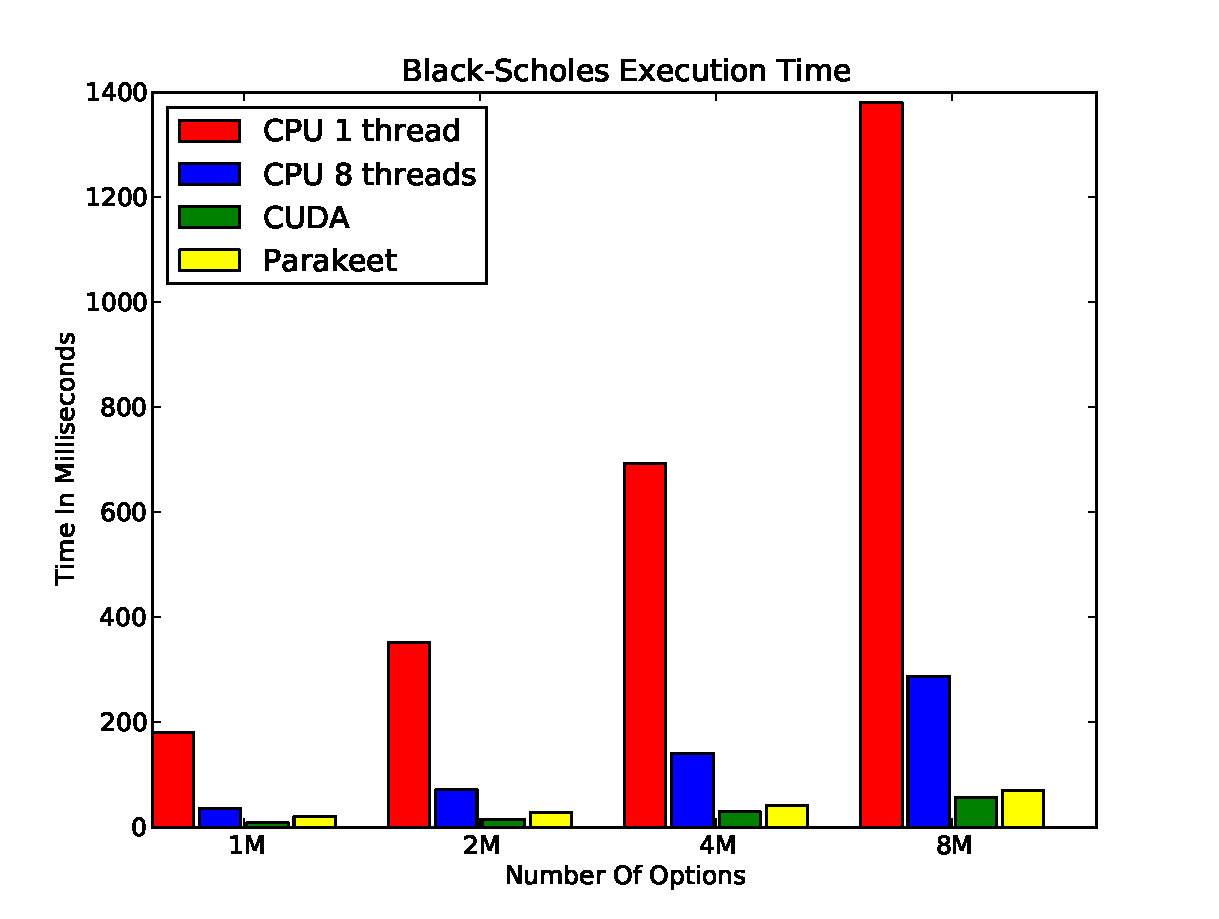
\includegraphics[scale=0.45]{BSWCPU.pdf}
\caption{Black Scholes Total Times}
\label{BSCPU}
\end{figure}


In Figure \ref{BSCPU}, we see the total run times of the various systems. These times include the time it takes to transfer data to and from the GPU in the GPU benchmarks.  As expected, Black Scholes performs very well on the GPU as compared with the CPU, since it is a purely data parallel benchmark.  We see that Parakeet performs very similarly to the hand-written CUDA version, with overheads decreasing as a percentage of the run time as the data sizes grow.  This is due to the fact that most of these overheads are fixed costs related to dynamic compilation.

\begin{figure}[h!]
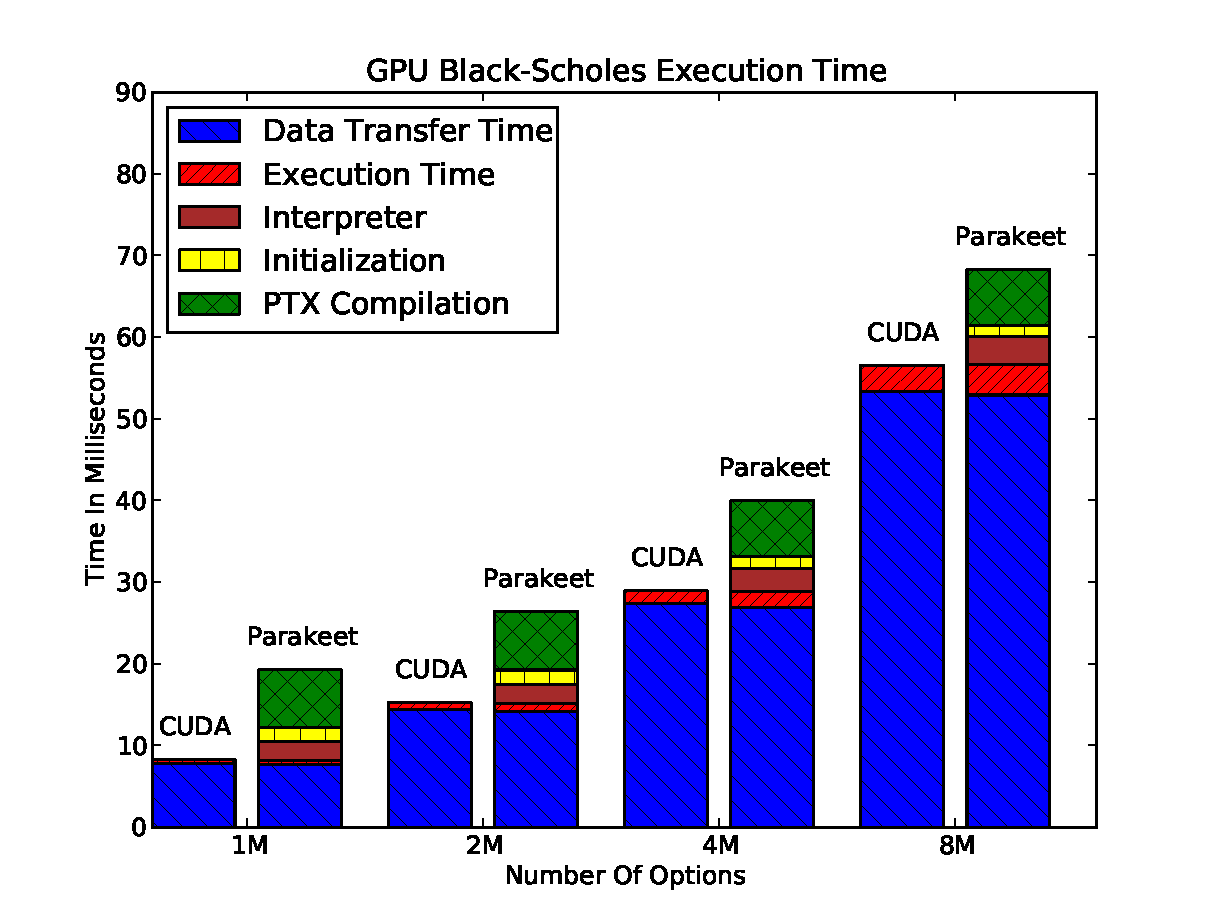
\includegraphics[scale=0.45]{BSNOCPU.pdf}
\caption{Black Scholes GPU Execution Times}
\label{BSGPU}
\end{figure}

In Figure \ref{BSGPU}, we break down Parakeet's performance as compared with the hand-written CUDA version.  The Parakeet run times range from 24\% to 2.4X slower than those of CUDA, with Parakeet performing better as the data size increases.  These results illustrate an important aspect of GPU acceleration, viz. that the cost of transferring data to and from the GPU's memory is rather expensive.  This large data transfer cost is, however, the same for Parakeet and CUDA.  The GPU programs that Parakeet generates are slightly less efficient than those of the CUDA version, with approximately 50\% higher run time on average.  However, the data transfer costs overwhelm the GPU execution times for Black Scholes, so this overhead isn't very important. 

 There are three other sources of overhead for Black Scholes that Parakeet introduces:
\begin{enumerate}
\item Initialization costs related to registering the Black Scholes function with the Parakeet runtime.
\item Time spent in the Parakeet IL interpreter.
\item The cost of running the JIT compiler on the generated PTX.
\end{enumerate}

The PTX compilation time is rather significant for this benchmark -- ranging from 33\% of the total runtime for the 1 million option case to roughly 10\% in the 8 million option case.  This cost can't be helped, but it is important to note that it as well as the initialization costs are only paid once per function since Parakeet caches the compiled version of the function.  Thus, in the case of workloads where a single function is repeatedly called, this costs will be insignificant.

\subsection{K-Means Clustering}
\label{results-k-means}

\begin{figure}
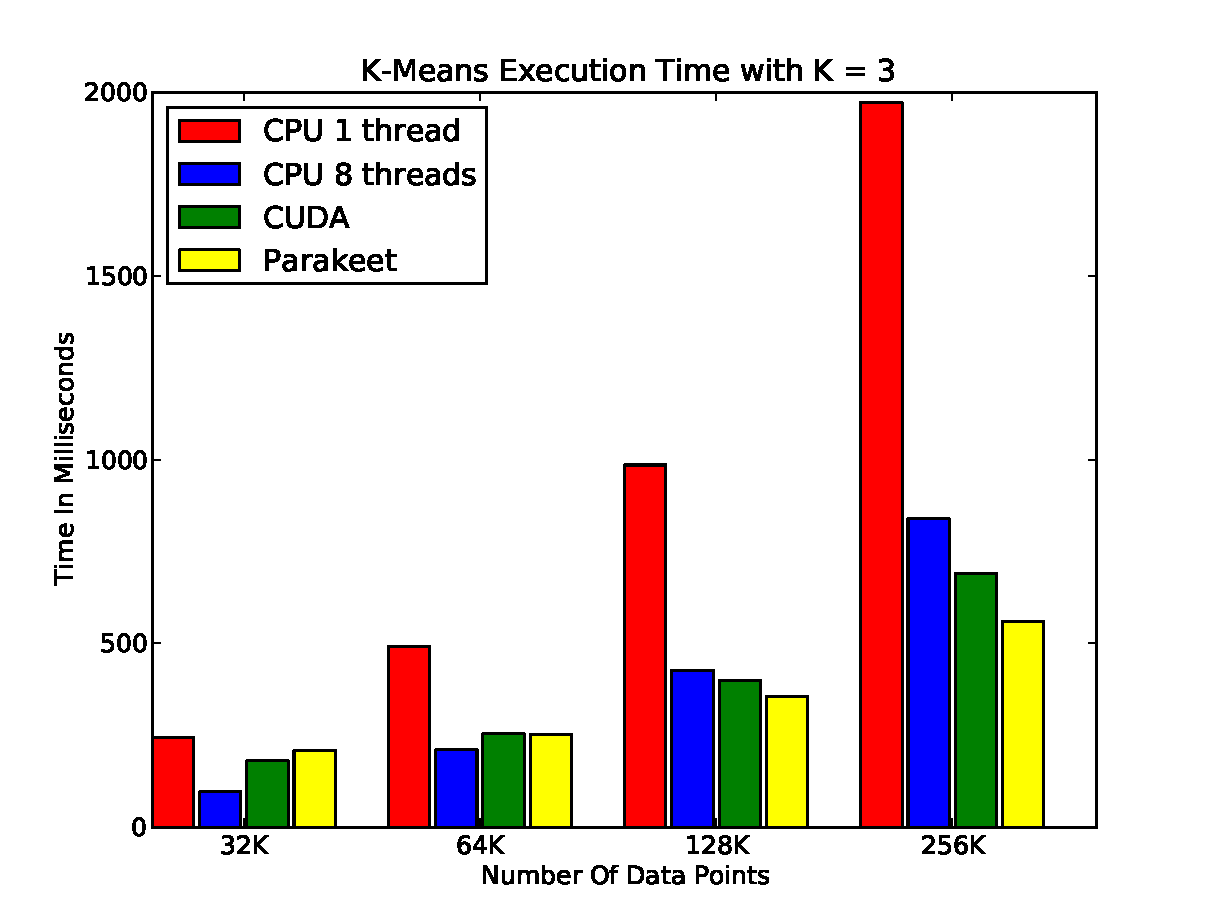
\includegraphics[scale=0.45]{KMCPUK3.pdf}
\caption{K-Means Total Times with 30 Features, K = 3}
\label{KMCPU3}
\end{figure}

We also tested Parakeet on K-Means clustering, a standard unsupervised learning algorithm.  K-Means is interesting as it is a fairly dense and complicated algorithm with loops and nested array operators.  Thus it serves to illustrate that Parakeet is a usable system for implementing real world programs.  K-Means has a number of parameters that can greatly affect run times and algorithmic characteristics.  These include: the number of data points being clustered; the number of clusters K; and the number of features (i.e.~the dimensionality of the data points).

In Figure \ref{KMCPU3}, we see the total run times of K-Means for the CPU and GPU versions with K = 3 clusters and 30 features on varying numbers of data points.  Here, the distinction between the GPU and the CPU is far less stark.  In fact, for two smaller numbers of data points the 8-thread CPU version actually outperforms the GPU.  More importantly for the present discussion, we see that on all but the smallest input size, Parakeet actually performs better than both the CPU and GPU versions.

The reason Parakeet is able to perform so well as compared with the CUDA version is due to the difference in how the two versions end up executing the code that computes the new average centroid for the newly computed clusters in each iteration.  The CUDA version brings the GPU-computed assignment vectors back to the CPU in order to perform this reduction, as it involves many poor memory accesses and so has the potential to perform poorly on the GPU.  Parakeet executes code to perform this function on the GPU instead, prefering to avoid the data transfer penalty.  For such a small number of clusters, the Parakeet method ends up performing far better.  For larger numbers of clusters, the fixed overhead of launching an individual kernel to average each cluster's points overwhelms the performance advantage the GPU gives and Parakeet ends up performing worse. While we don't take advantage of it yet, this illustrates the potential for us to use dynamic information to get the best of both worlds.  In the future, in the case of a small number of clusters, Parakeet could execute the averaging code on the GPU, while for larger numbers, it could use a CPU implementation.

\begin{figure}
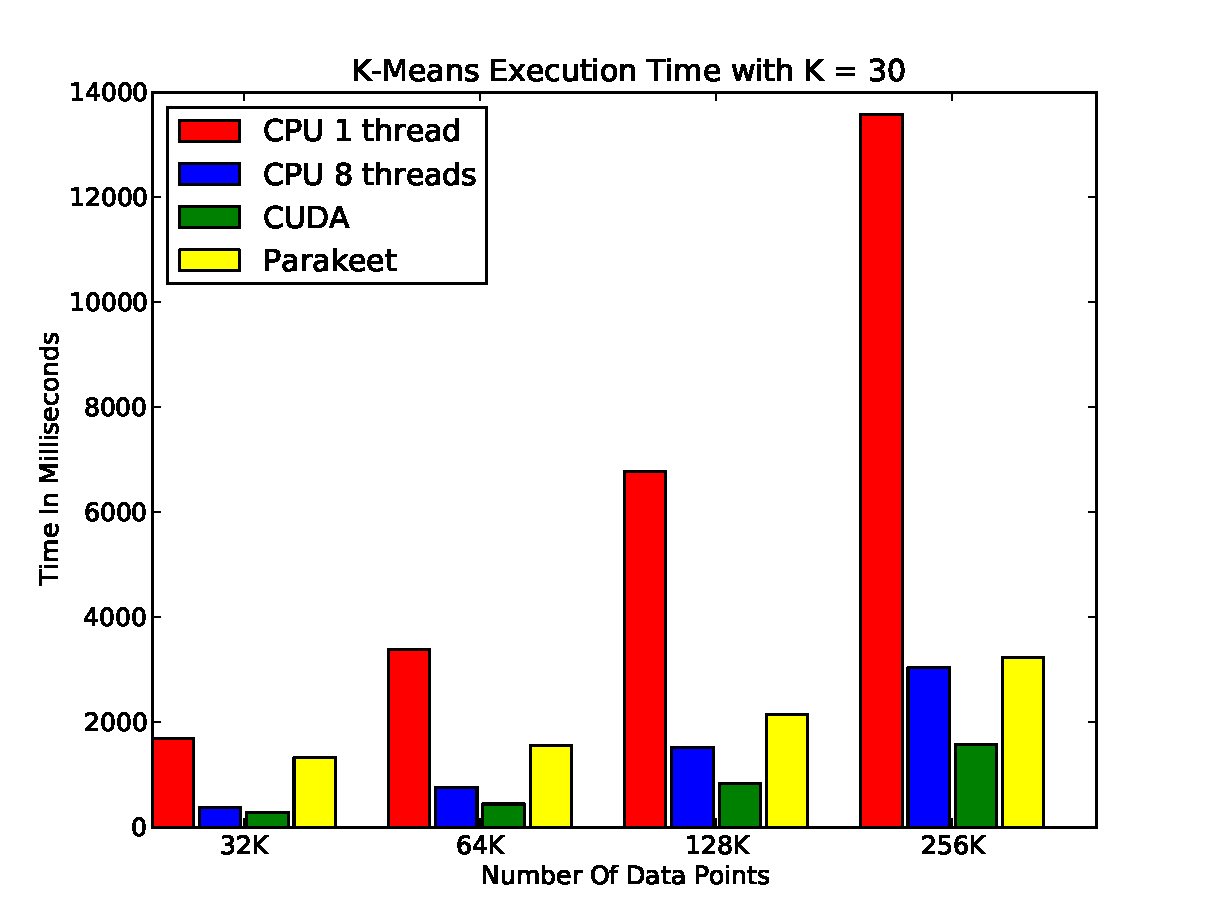
\includegraphics[scale=0.45]{KMCPUK30.pdf}
\caption{K-Means Total Times with 30 Features, K = 30}
\label{KMCPU30}
\end{figure}

In Figure \ref{KMCPU30}, we present the run times of K-Means for 30 features and K = 30 clusters.  In this case, the hand-written CUDA version performs best in all cases, though its advantage over the CPU increases and its advantage over Parakeet decreases with increasing data size.  As discussed, the Parakeet implementation suffers from the poorly performing averaging computation that it executes on the GPU, with a best case of an approximate 2X slowdown over the CUDA version.  However, Parakeet exhibits the best scaling of any of the implementations, and would likely close the gap even further at larger data sizes.

\begin{figure}
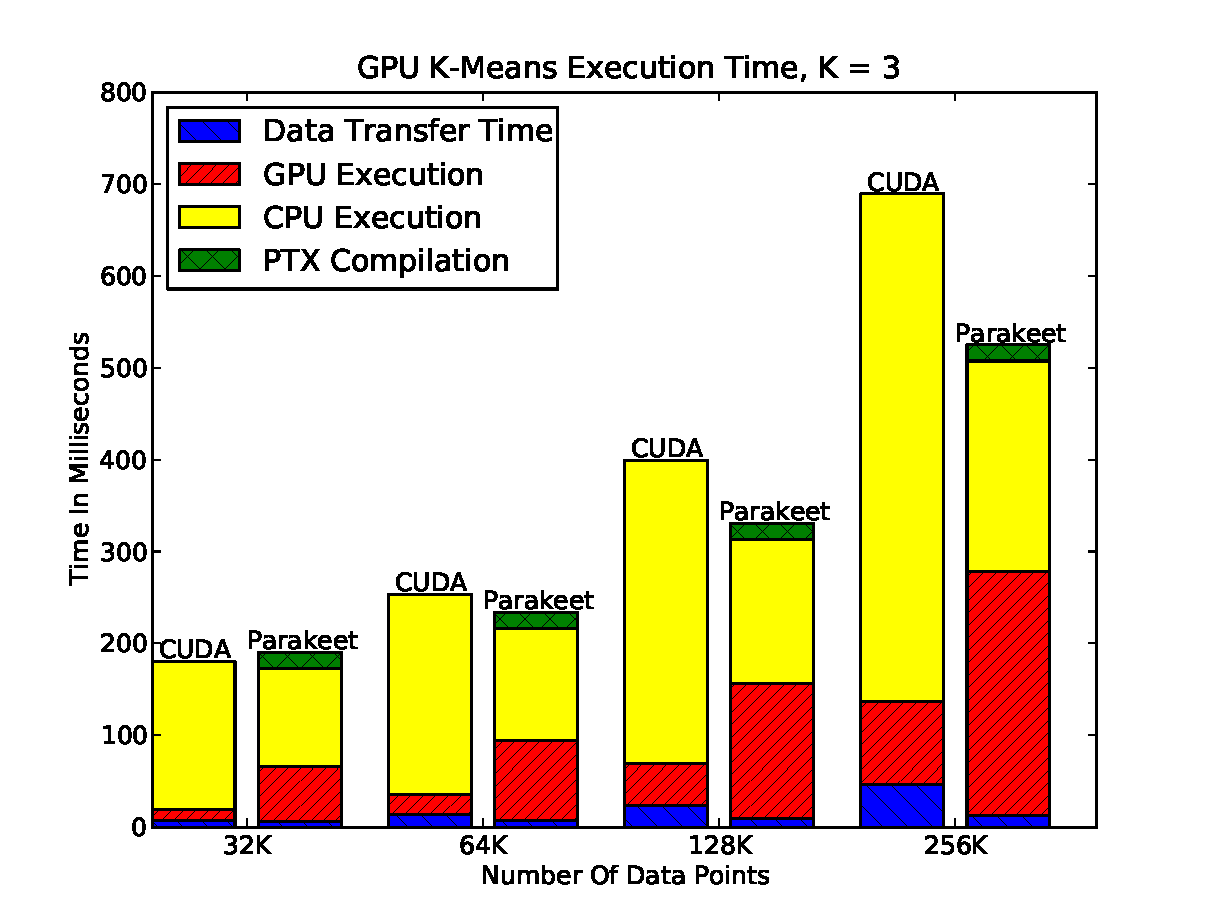
\includegraphics[scale=0.45]{KMGPU.pdf}
\caption{K-Means GPU Times with 30 Features, K = 3}
\label{KMGPU}
\end{figure}

In Figure \ref{KMGPU}, we see a breakdown of the run times for CUDA and Parakeet on the K = 3 clusters case.  We can see that this benchmark is much more compute bound than Black Scholes, with the memory transfer costs contributing a much smaller percentage of the overall run time.  Both Parakeet and the CUDA version use the CPU to perform a significant amount off the computation.  The CUDA version uses the CPU to compute the averages of the new clusters in each iteration, while Parakeet spends a lot of time in the interpreter launching many GPU kernels and performing garbage collection of GPU memory.  Even though the performance of Parakeet is fantastic, we imagine that with some more tuning we could push this gap even further.

K-Means clustering illustrates a key aspect of our approach: the ability to exploit dynamic information to tailor code generation and execution.  When calculating centroids, we have a $\MAP$ operator using a nested function that in turns contains array operators.  Our interpreter is able to make the most efficient choice regarding execution placement: the outer $\MAP$, since it is applied to a small array of integers and involves little computation of its own, gets executed on the CPU as a loop.  The inner function, which since it has dense computation applied to large inputs, gets synthesized into a kernel that is repeatedly launched.  This type of dynamic decision based on data size would not be possible in a static environment.  In addition, Parakeet uses transposition to a column-major data layout (see Section \ref{datalayout}) in order to greatly improve the performance of this benchmark -- transposition results in an average 12.5X speedup of K-Means clustering as a whole. The function which calculates centroid assignments is implemented as a map kernel where each thread is responsible for calculting the distance from its data point to every centroid. The Parakeet runtime identifies maps over 2D structures with nested maps over the rows, and transposes their inputs. This optimization is crucial for attaining coalesced memory accesses, and its absence can be ruinous for GPU performance.  Since a transposed data matrix can be reused across loop iterations, the relative overhead of performing a transposition is very low.

\section{Related Work}
\label{RelatedWork}
The use of graphics hardware for non-graphical computation has a  long history~\cite{Leng90}, though convenient frameworks for general purpose GPU programming have only recently emerged. The first prominent GPU backend for a general purpose language was ``Brook for GPUs'' \cite{Buck04}. The Brook language extended C with ``kernels'' and ``streams'', exposing a programming model similar to what is now found in CUDA and OpenCL.

Microsoft's Accelerator~\cite{Tard06} was the first project to use high level (collection-oriented) language constructs as a basis for GPU execution. Accelerator is a declarative GPU language embedded in C\# which creates a directed acyclic graph of LINQ operations -- such as filtering, grouping, and joining -- and compiles them to (pre-CUDA) shader programs. Accelerator's programming model does not support function abstractions (only expression trees) and its only underlying parallelism construct is limited to the production of $\MAP$-like kernels.

Three more recent projects all translate domain specific embedded array languages to CUDA backends:
\begin{itemize}
\item \textbf{Nikola}~\cite{Main10} is a first-order array-oriented language embedded within Haskell. Nikola provides a convenient syntax for expressing single-kernel computations, but requires the programmer to manually coordinate computations which require multiple kernel launches. Nikola also does not support partially applied functions and its parallelization scheme, which first serializes array operators into loops and then parallelizes loop iterations, seems ill-suited for complex array operations.

\item \textbf{Accelerate}~\cite{Chak11} is also an embedded array language within Haskell. Unlike Nikola, Accelerate does allow the expression of computations which span multiple kernel launches. Accelerate also has a much richer set of array operators (including the higher-order trio $\MAP$, $\REDUCE$, $\SCAN$). Accelerate, however, does not seem to support closures or the nesting of array operators. Accelerate's backend is similar to ours in that they use a simple interpreter whose job is to initiate skeleton-based kernel compilation, transfer data to and from the GPU, and to perform simple CPU-side computations.

\item \textbf{Copperhead}~\cite{Cata11} parallelizes a statically typed purely functional array subset of Python through the dynamic compilation/execution of CUDA kernels. Copperhead supports nested array computations, and even has a sophisticated notion of where these computations can be scheduled. In addition
to sequentializing nested array operators within CUDA kernels (as done in Parakeet), Copperhead can also share the work of a nested computation between all the threads in CUDA block. Unfortunately, Copperhead does not utilize any dynamic information (such as size) when making these scheduling decisions and
thus must rely on user annotations. Copperhead's compiler generates kernels through parameterization of operator-specific C++ template classes. By using C++ as their backend target, Copperhead has been able to easily integrate the Thrust ~\cite{Hobe10} GPGPU library and to offload the bulk of their code optimizations onto a C++ compiler. Runtime generation of templated C++ can, however, be a double-edged sword. Copperhead experiences the longest compile times of any project mentioned here (orders of magnitude longer than the compiler overhead of Parakeet).
\end{itemize}
Unlike the three approaches mentioned above, Parakeet does not require its source language to be purely functional nor statically typed. Being able to program in a dynamically typed language seems particularly important for array computations, since static type systems are generally unable to support the syntactic conveniences which make array programming appealing in the first place.

\section{Conclusion}
\label{Conclusion}

Parakeet allows the programmer to write in a high level sequential array language while taking advantage of the acceleration potential of using GPUs as coprocessors. Parakeet automatically synthesizes and executes very efficient GPU programs from the high level code while transparently moving data back and forth to the GPU's memory and performing GPU memory garbage collection. Parakeet includes a series of optimizations to generate more efficient GPU programs, including array operator fusion, data transposition, and the use of texture memory on the GPU.  Parakeet is a usable system in which complex programs can be written and executed efficiently.  On two benchmark programs, Parakeet delivers performance very competitive with even hand-tuned GPU implementations without impacting the interactivity of the source language interpreter environment.

In future work, we hope to support both more front ends and more back ends.  At the moment, we are nearing completion of a front end for Python's NumPy, and we plan to build a front end for Matlab as well.  Further, we envision building a back end for multicore CPUs, likely targeting LLVM~\cite{Latt02}, which will allow us to simultaneously take advantage of the particular strengths of both types of processors.

In addition, we plan to increase efficiency by iteratively tuning components of hierarchical algorithms, splitting data inputs to take advantage of more of the texturing hardware, and doing more to overlap computation with data transfers.

{\small
\bibliographystyle{acm}
\bibliography{../Parallelism}{}
}
\end{document}
